% !TeX root = ./main.tex
\section{ansatz}
\subsection{Recurrent Neural Network}
\begin{equation}
    \begin{split}
    \Psi(\mathbf{x}) = \sum_{\mathbf{x}}\psi(\mathbf{x})\ket{\mathbf{x}} &= \sum_{\mathbf{x}}\sqrt{P(\mathbf{x})}\ket{\mathbf{x}} \quad \text{Real} \\
    \text{or} & = \sum_{\mathbf{x}}\exp{[i\phi(\mathbf{x})]}\sqrt{P(\mathbf{x})}\ket{\mathbf{x}} \quad \text{Complex}
    \end{split}
\end{equation}
Conditional probability\cite{HibatAllah2020} $P_i$:
\begin{equation}
    \begin{split}
    P_i& = y_i^{(1)} \cdot x_i \\
    y_i^{(1)} & = \mathbf{softmax}(\underbrace{U^{(1)}\mathbf{h}_i + \mathbf{c}^{(1)}}_{\text{Linear Layers-1}}) \\
    \mathbf{softmax}(v_n) & = \frac{\exp{(v_n)}}{\sum_i \exp{(v_i)}}
    \end{split}
\end{equation}
phase:
\begin{equation}
    \begin{split}
    \phi_i & = y_i^{(2)} \cdot x_i \\
    y_i^{(2)} & = \pi \mathbf{softsign}(\underbrace{U^{(2)}\mathbf{h}_i + \mathbf{c}^{(2)}}_{\text{Linear Layers-2}}) \\
    \mathbf{softsign}(x) & = \frac{x}{1 + x} \in (-1, 1)
    \end{split}
\end{equation}
这里Linear Layers-1和Linear Layers-2可以共用同一套参数.\\
$x_i$是\textbf{ont-hot encoding}, 对于spin $\frac{1}{2}$体系:
\begin{equation}
    x_i \in (1, 0) \ or \ (0, 1)
\end{equation}
对于有\textit{N}个轨道的体系有
\begin{equation}
    \begin{split}
    P(\mathbf{x}) & = \prod_{i=1}^N P_i\\
    \phi(\mathbf{x}) &= \sum_{i=1}^N \phi_i
    \end{split}
\end{equation}

\subsection{Restricted Boltzmann Machine}
\begin{equation}
    \begin{split}
    \psi_{\theta}(\mathbf{x}) & = \textcolor{teal}{\exp}{\sum_{j=1}^{N_v}a_jx_j} \times 
        \prod_i^{N_h}\textcolor{violet}{2\cosh}(b_i + \sum_{j=1}^{N_v}W_{ij}x_j) \\
        \text{or} & = \prod_i^{N_h}\textcolor{violet}{2\cos}(b_i + \sum_{j=1}^{N_v}W_{ij}x_j) \quad 
        \textbf{cos-type}\\
        \text{or} & = \textcolor{teal}{\tanh}{\sum_{j=1}^{N_v}a_jx_j} \times 
        \prod_i^{N_h}\textcolor{violet}{2\cosh}(b_i + \sum_{j=1}^{N_v}W_{ij}x_j) \quad
        \textbf{tanh-type}
    \end{split}
\end{equation}
where $x_j$ represents the visible spin, $h_i$ the hidden spin and $W_{ij}$ weight parameters.
$N_v$, $N_h$ are the number of visible , hidden spins and weight respectively.\\
default:
\begin{equation}
    \alpha = N_h/N_v
\end{equation}

\subsubsection{AR-RBM}
\textit{K}-th sites\ ($1 \leq K \leq n_{sorb}=N_v$), $\mathbf{W}_K : (N_h, K)$\cite{bortone2023impact}
\begin{equation}
    \begin{split}
    \mathbf{x}_{K1} & = (x_0, \cdots, x_{K-1}, 1) \\
    \mathbf{x}_{K2} & = (x_0, \cdots, x_{K-1}, 0) \\
    \end{split}
\end{equation}

\begin{equation}
    \begin{split}
    \psi_{\theta}(\mathbf{x}_{K1}) & = \prod_{i}^{N_h}\textcolor{violet}{2\cos}
        (\Theta +W_{i\textcolor{blue}{K}}x_{\textcolor{blue}{K}1}) \\
    % (b_i + \sum_{\textcolor{blue}{k}=1}^{\textcolor{blue}{K}}W_{i\textcolor{blue}{k}}x_{\textcolor{blue}{k}}) \\
    \psi_{\theta}(\mathbf{x}_{K2}) & = \prod_{i}^{N_h}\textcolor{violet}{2\cos}
        (\Theta +W_{i\textcolor{blue}{K}}x_{\textcolor{blue}{K}2})\\
    % (b_i + \sum_{\textcolor{blue}{k}=1}^{\textcolor{blue}{K}}W_{i\textcolor{blue}{k}}x_{\textcolor{blue}{k}}) \\
    \Theta & = b_i + \sum_{\textcolor{blue}{k}=1}^{\textcolor{blue}{K-1}}W_{i\textcolor{blue}{k}}x_{\textcolor{blue}{k}} \\
    \end{split}
\end{equation}

\noindent Normalized $\psi_{\theta}(\mathbf{x}_{K1}), \psi_{\theta}(\mathbf{x}_{K2})$
to $\widetilde{\psi}_{\theta}(\mathbf{x}_{K1}), \widetilde{\psi}_{\theta}(\mathbf{x}_{K2})$:
\begin{equation}
    \psi_{\theta}(\mathbf{x}) = \prod_{i=1}^{N_v}\frac{\widetilde{\psi}_i(x_i|\mathbf{x}_{<i})}
    {\sqrt{\sum_{x^\prime = 0}^{D-1}\vert \widetilde{\psi}_i(x^\prime |\mathbf{x}_{<i})\vert^2}}
    \enskip \mathrm{s.t.} ~ D = 2
\end{equation}

For two sites:
\begin{equation}
    \begin{split}
    \mathbf{x}_{K1} & = (x_0, \cdots, x_{K-2}, 0, 0) \\
    \mathbf{x}_{K2} & = (x_0, \cdots, x_{K-2}, 1, 0) \\
    \mathbf{x}_{K3} & = (x_0, \cdots, x_{K-2}, 0, 1) \\
    \mathbf{x}_{K4} & = (x_0, \cdots, x_{K-2}, 1, 1) \\
    \end{split}
\end{equation}

\begin{equation}
    \begin{split}
    \psi_{\theta}(\mathbf{x}_{K1}) & = \prod_{i}^{N_h}\textcolor{violet}{2\cos}
        (\Theta +W_{i\textcolor{blue}{K}-1}x_{\textcolor{blue}{K}1-1} + W_{i\textcolor{blue}{K}}x_{\textcolor{blue}{K}1}) \\
    \psi_{\theta}(\mathbf{x}_{K2}) & = \prod_{i}^{N_h}\textcolor{violet}{2\cos}
        (\Theta +W_{i\textcolor{blue}{K}-1}x_{\textcolor{blue}{K}2-1} + W_{i\textcolor{blue}{K}}x_{\textcolor{blue}{K}2})\\
    \psi_{\theta}(\mathbf{x}_{K2}) & = \prod_{i}^{N_h}\textcolor{violet}{2\cos}
        (\Theta +W_{i\textcolor{blue}{K}-1}x_{\textcolor{blue}{K}3-1} + W_{i\textcolor{blue}{K}}x_{\textcolor{blue}{K}3})\\
    \psi_{\theta}(\mathbf{x}_{K2}) & = \prod_{i}^{N_h}\textcolor{violet}{2\cos}
        (\Theta +W_{i\textcolor{blue}{K}-1}x_{\textcolor{blue}{K}4-1} + W_{i\textcolor{blue}{K}}x_{\textcolor{blue}{K}4})\\
    \Theta & = b_i + \sum_{\textcolor{blue}{k}=1}^{\textcolor{blue}{K-2}}W_{i\textcolor{blue}{k}}x_{\textcolor{blue}{k}} \\
    \end{split}
\end{equation}

% \begin{figure}[htp]
%     \centering
%     \includegraphics[width=0.5\textwidth]{AR-RBM.pdf}
%     \caption{AR-RBM测试:\ce{H4}-1.40, $\alpha = 2, \mathrm{random\ seed} = 112123, AE= 0.00001$}
% \end{figure}

\subsection{Transformer}
\textcolor{darkred}{\textbf{TODO:}} ref:\cite{zhang2023transformer,wu2023nnqs}

\subsection{Constraints Fock space \texorpdfstring{$\rightarrow$}{→} FCI space}

Molecular system determines satisfy:
\begin{equation}
    \begin{split}
    n_{\alpha} + n_{\beta} & = n_e \\
    n_{\alpha} - n_{\beta} & = C \\
    \end{split}
\end{equation}

the configuration $x \in \{0, 1\}^{N}$, (1: occupied, 0: unoccupied, N: spin-orbitals),
k-th spin-orbitals satisfy:
\begin{equation}
    \begin{split}
        n_{\alpha} - \left(\frac{N}{2} - k//2\right) &
            \leq n_{\uparrow} = \sum_{j=0}^{k//2}x_{2j} \leq n_{\alpha} \\
        n_{\beta} - \left(\frac{N}{2} - k//2\right) &
            \leq n_{\downarrow} = \sum_{j=0}^{k//2}x_{2j+1} \leq n_{\beta} \\
    \end{split}
\end{equation}
so, when k is even number ($n_{\uparrow}$ \textbf{dose not include} k-th spin-orbitals for \textbf{sampling convenience}):
\begin{equation}
    n_{\alpha} - \left(\frac{N}{2} - k//2\right) < n_{\uparrow} \quad n_{\alpha} > n_{\uparrow} \label{cond1}
\end{equation}
when k is old number  ($n_{\downarrow}$ \textbf{dose not include} k-th spin-orbitals for \textbf{sampling convenience}):
\begin{equation}
    n_{\beta} - \left(\frac{N}{2} - k//2\right) < n_{\downarrow} \quad n_{\beta} > n_{\downarrow} \label{cond2}
\end{equation}
Eqs\ \ref{cond1},\ \ref{cond2} can get bool array $cond_{idx}$
\begin{equation}
 cond_{idx} \in \textcolor{blue}{[0, 1]} \ \textcolor{violet}{[1, 0]}\ \textcolor{teal}{[1, 1]},
\end{equation}
which mean the next spin-orbitals must be \textcolor{blue}{unoccupied[0]},
\textcolor{violet}{occupied[1]} and \textcolor{teal}{unoccupied or occupied[0]/[1]}.\\
adapt before probability 
\begin{equation}
    prob_0 = [p_0, p_1] \ s.t.\ p_0 + p_1 \equiv 1.0
\end{equation}
($p_0, p_1$ are probability of the spin-orbitals is occupied and unoccupied)\\
adapt after probability
\begin{equation}
prob_1 =[p_0, p_1] * cond_{idx} = [p_0^{\prime}, p_1^{\prime}] 
    \ s.t.\ p_0^{\prime} + p_1^{\prime} \equiv 1.0 \ (\textrm{Normalized})
\end{equation}
\indent The above is for the case of one spin-orbitals, however, 
the case of two spin-orbitals is \textbf{convoluted}.
Eqs\ \ref{cond1} and \ref{cond2} can get bool array $cond_{idx}\alpha, cond_{idx}\beta$:
\begin{equation}
    \begin{split}
    cond_{idx}\alpha & \in \textcolor{blue}{[0, 1]} \ \textcolor{violet}{[1, 0]}\ \textcolor{teal}{[1, 1]} \\
    cond_{idx}\beta & \in \textcolor{blue}{[0, 1]} \ \textcolor{violet}{[1, 0]}\ \textcolor{teal}{[1, 1]} 
    \end{split}
\end{equation}
combine $\textcolor{darkred}{[cond_{idx}\alpha, cond_{idx}\beta]}$:
\begin{equation}
    \begin{split}
        & [0, 1, 0, 1], [0, 1, 1, 0], [0, 1, 1, 1] \\
        & [1, 0, 0, 1], [1, 0, 1, 0], [1, 0, 1, 1] \\
        & [1, 1, 0, 1], [1, 1, 1, 0], [1, 1, 1, 1] \\
    \end{split}
\end{equation}
means $[\alpha, \beta]$:
\begin{equation}
    \begin{split}
        [0, 0], & [0, 1], ([0, 1], [0, 0]) \\
        [1, 0], & [1, 1], ([1, 1], [1, 0]) \\
        ([1, 0], [0, 0]), & ([1, 1], [0, 1]), ([0, 0], [1, 0], [0, 1], [1, 1])
    \end{split}
\end{equation}
convert to Binary Number:
\begin{equation}
    \begin{split}
        &0, 2, (0, 2) \\
        &1, 3, (1, 3) \\
        &(1, 0), (3, 2) , (0, 1, 2, 3)
    \end{split}
\end{equation}
so the merged bool array $merged$:
\begin{equation}
    \begin{split}
        &[1, 0, 0, 0], [0, 0, 1, 0], [1, 0, 1, 0] \\
        &[0, 1, 0, 0], [0, 0, 0, 1], [0, 1, 0, 1] \\
        &[1, 1, 0, 0], [0, 0, 1, 1], [1, 1, 1, 1]
    \end{split}
\end{equation}
\noindent Adapt before probability
\begin{equation}
    prob_0 = [p_0, p_1, p_2, p_3] \ s.t.\ p_0 + p_1 + p_2 + p_3 \equiv 1.0
\end{equation}
($p_0, p_1, p_2, p_3$ are the probability of $[0, 0], [1, 0], [0, 1], [1, 1]$($[\alpha, \beta]$))\\
Adapt after probability
\begin{equation}
    \begin{split}
        prob_1 =[p_0, p_1, p_2, p_3] * merged & = [p_0^{\prime}, p_1^{\prime}, p_2^{\prime}, p_3^{\prime}] \\
        & \ s.t.\ p_0^{\prime} + p_1^{\prime} + p_2^{\prime} + p_3^{\prime} \equiv 1.0 \ (\textrm{Normalized})
    \end{split}
\end{equation}
Therefore, \textbf{make charts} and $\textcolor{darkred}{[cond_{idx}\alpha, cond_{idx}\beta]}$
is converted to Binary Number:
\begin{equation}
    charts =
    \begin{cases}
        10 & \Rightarrow [1, 0, 0, 0] \\
        6 & \Rightarrow [0, 0, 1, 0] \\
        14 & \Rightarrow [1, 0, 1, 0] \\
        9 & \Rightarrow [0, 1, 0, 0] \\
        5 & \Rightarrow [0, 0, 0, 1] \\
        13 & \Rightarrow [0, 1, 0, 1] \\
        11 & \Rightarrow [1, 1, 0, 0] \\
        7 & \Rightarrow [0, 0, 1, 1] \\
        15 & \Rightarrow [1, 1, 1, 1] \\
    \end{cases}
\end{equation}

\subsection{Excluded partial determines}
\begin{figure}[htp]
    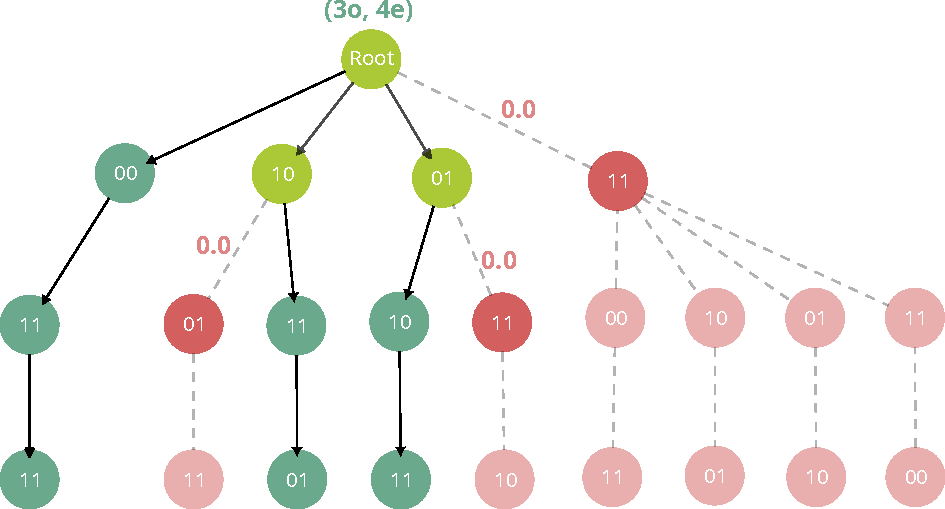
\includegraphics[width=0.90\textwidth]{../remove-det}
    \caption*{Quadtree excluding partial determines}
\end{figure}